\section{Experiments}
\begin{table*}[ht]
\centering
\footnotesize
\setlength{\tabcolsep}{0.4em}
\caption{{Few-shot detection performance (mAP50) on the PASCAL VOC dataset.} We evaluate the performance on three different sets of novel classes. Our approach consistently outperforms baseline methods by a large margin (about 2$\sim$20 points), especially when the number of shots is low. FRCN stands for Faster R-CNN. \model w/ cos is our approach with a cosine similarity based box classifier. \vspace{1mm}
}
\adjustbox{width=\linewidth}{
\begin{tabular}{l|c|ccccc|ccccc|ccccc}
\toprule
\multirow{2}{*}{Method / Shot} & \multirow{2}{*}{Backbone} & \multicolumn{5}{c|}{Novel Set 1} & \multicolumn{5}{c|}{Novel Set 2} & \multicolumn{5}{c}{Novel Set 3} \\ 
&  & 1     & 2     & 3    & 5    & 10   & 1     & 2     & 3    & 5    & 10   & 1     & 2     & 3    & 5    & 10   \\ \midrule
\bs{}~\cite{kang2019few}   &  \multirow{5}{*}{YOLOv2}  & 0.0   & 0.0   & 1.8  & 1.8  & 1.8  & 0.0   & 0.1   & 0.0  & 1.8  & 0.0    & 1.8   & 1.8   & 1.8  & 3.6  & 3.9  \\ %\hline
\bbsshort{}~\cite{kang2019few}  & & 3.2   & 6.5   & 6.4  & 7.5  & 12.3 & 8.2   & 3.8   & 3.5  & 3.5  & 7.8  & 8.1   & 7.4   & 7.6  & 9.5  & 10.5 \\ %\hline
\bbs{}~\cite{kang2019few}  &  & 6.6   & 10.7  & 12.5 & 24.8 & 38.6 & 12.5  & 4.2   & 11.6 & 16.1 & 33.9 & 13.0  & 15.9  & 15.0 & 32.2 & 38.4 \\ 
FSRW~\cite{kang2019few}  &  & 14.8  & 15.5  & 26.7 & 33.9 & 47.2 & 15.7  & 15.3  & 22.7 & 30.1 & 40.5 & 21.3  & 25.6  & 28.4 & 42.8 & 45.9 \\ 
MetaDet~\cite{wang2019meta} & & 17.1 & 19.1 & 28.9 & 35.0 & 48.8 & 18.2 & 20.6 & 25.9 & 30.6 & 41.5 & 20.1 & 22.3 & 27.9 & 41.9 & 42.9 \\ \midrule
FRCN+joint~\cite{wang2019meta} & \multirow{3}{*}{FRCN w/VGG16} & 0.3 & 0.0 & 1.2 & 0.9 & 1.7 & 0.0 & 0.0 & 1.1 & 1.9 & 1.7 & 0.2 & 0.5 & 1.2 & 1.9 & 2.8\\
FRCN+joint-ft~\cite{wang2019meta} & & 9.1 & 10.9 & 
13.7 & 25.0 & 39.5 & 10.9 & 13.2 & 17.6 & 19.5 & 36.5 & 15.0 & 15.1 & 18.3 & 33.1 & 35.9 \\
MetaDet~\cite{wang2019meta} &  & 18.9 & 20.6 & 30.2 & 36.8 & 49.6 & 21.8 & 23.1 & 27.8 & 31.7 & 43.0 & 20.6 & 23.9 & 29.4 & 43.9 & 44.1 \\ \midrule
FRCN+joint~\cite{yan2019meta} & \multirow{4}{*}{FRCN w/R-101} & 2.7 & 3.1 & 4.3 & 11.8 & 29.0 & 1.9 & 2.6 & 8.1 & 9.9 & 12.6 & 5.2 & 7.5 & 6.4 & 6.4 & 6.4 \\
FRCN+ft~\cite{yan2019meta} &  & 11.9 & 16.4 & 
29.0 & 36.9 & 36.9 & 5.9 & 8.5 & 23.4 & 29.1 & 28.8 & 5.0 & 9.6 & 18.1 & 30.8 & 43.4 \\
FRCN+ft-full~\cite{yan2019meta} &  & 13.8 & 19.6 
& 32.8 & 41.5 & 45.6 & 7.9 & 15.3 & 26.2 & 31.6 & 39.1 & 9.8 & 11.3 & 19.1 & 35.0 & 45.1 \\
Meta R-CNN~\cite{yan2019meta} &  & 19.9 & 25.5 & 35.0 & 45.7 & 51.5 & 10.4 & 19.4 & 29.6 & 34.8 & \textbf{45.4} & 14.3 & 18.2 & 27.5 & 41.2 & 48.1 \\ \midrule
% Two-stage ft w/ FC & Faster R-CNN w/ ResNet-101 & 18.7 & 27.4 & 37.3 & 49.2 & 52.3 & 6.5 & 19.9 & 25.4 & 25.5 & 27.4 &  27.7 & 33.6 & 42.5 & 48.7 & \textbf{50.2}\\ 
% Two-stage ft w/ cos & Faster R-CNN w/ ResNet-101 & 39.8 & 35.9 & 44.7 & 55.7 & 56.0 & 22.0 & 26.6 & 34.0 & 35.3 & 38.9 & 30.8 & 34.8 & 42.8 & 49.5 & 49.8 \\
% FRCN+joint (Ours) & \multirow{2}{*}{FRCN w/R-101} & 0.0 &  &  &  &  &  &  &  &  &  &  &  &  &  &  \\
FRCN+ft-full (Our Impl.) &  & 15.2 & 20.3 & 29.0 & 40.1 & 45.5 & 13.4 & 20.6 & 28.6 & 32.4 & 38.8 & 19.6 & 20.8 & 28.7 & 42.2 & 42.1 \\
\rowcolor{Gray} \model w/ fc (Ours) &  & 36.8 & 29.1 & 43.6 & \textbf{55.7} & \textbf{57.0} & 18.2 & \textbf{29.0} & 33.4 & \textbf{35.5} & 39.0 & 27.7 & 33.6 & 42.5 & 48.7 & \textbf{50.2} \\
\rowcolor{Gray} \model w/ cos (Ours) & \multirow{-3}{*}{FRCN w/R-101} & \textbf{39.8} & \textbf{36.1} & \textbf{44.7} & \textbf{55.7} & 56.0 & \textbf{23.5} & 26.9 & \textbf{34.1} & 35.1 & 39.1 & \textbf{30.8} & \textbf{34.8} & \textbf{42.8} & \textbf{49.5} & 49.8 \\
\bottomrule
\end{tabular}}
\label{tab:main_voc}
\end{table*}
In this section, we conduct extensive comparisons with previous methods on the existing 
few-shot object detection benchmarks using COCO, where our approach can obtain
about 2$\sim$20 points improvement in all settings (Section~\ref{sec:exist_benchmark}). We then introduce a new benchmark on three datasets (COCO and LVIS) with revised evaluation protocols to address the unreliability of previous benchmarks (Section~\ref{sec:revised_bench}). We also provide various ablation studies and visualizations in Section~\ref{sec:vis}. 

\minisection{Implementation details.}
% All of our models are implemented on the Detectron2 framework \cite{wu2019detectron2}.
We use Faster R-CNN~\cite{ren2015faster} as our base detector and Resnet-101~\cite{he2016deep} with a Feature Pyramid Network~\cite{lin2016feature} as the backbone.
% For hyperparameters related to the model architecture, we use the default parameters provided by Detectron2.
All models are trained using SGD with a mini-batch size of 16, momentum of 0.9, and weight decay of 0.0001.
A learning rate of 0.02 is used during base training and 0.001 during few-shot fine-tuning.
For more details, the code is available at~\url{https://github.com/ucbdrive/few-shot-object-detection}.

\subsection{Existing few-shot object detection benchmark}
\label{sec:exist_benchmark}
% We first evaluate our approach on two existing few-shot object detection benchmarks, PASCAL VOC \cite{pascal-voc-2007, pascal-voc-2012} and COCO \cite{Lin2014MicrosoftCC}.
% We use the same evaluation protocol as previous works \cite{kang2019few, yan2019meta, wang2019meta}, which we will describe next.
\minisection{Existing benchmarks.} 
Following the previous work~\cite{kang2019few,yan2019meta,wang2019meta}, we 
first evaluate our approach on PASCAL VOC 2007+2012 and COCO, using the same data splits and training examples provided by ~\citet{kang2019few}.
% \footnote{code and data at \url{https://github.com/bingykang/Fewshot_Detection}}. 
For the few-shot PASCAL VOC dataset,  the 20 classes are randomly divided into 15 base classes and 5 novel classes, where the novel classes have $K=1,2,3,5,10$ objects per class sampled from the combination of the trainval sets of the 2007 and 2012 versions for training. Three random split groups are considered in this work. PASCAL VOC 2007 test set is used for evaluation. For COCO, the 60 categories disjoint with PASCAL VOC are used as base classes while the remaining 20 classes are used as novel classes with $K=10, 30$.  For evaluation metrics, AP50 (matching threshold is 0.5) of the novel classes is used on PASCAL VOC and the COCO-style AP of the novel classes is used on COCO. 
% On PASCAL VOC, we use the train/val sets in VOC 2007 and 2012 for training and the VOC 2007 test set for evaluation.
% To construct the few-shot setting, we randomly split the 20 object categories into 15 as the base categories and the remaining 5 as the novel categories, and we evaluate on three different random splits.
% On COCO, we use 5k images from the validation set for evaluation and the remaining images from the train/val sets for training.
% From the 80 object categories, we set the same 20 categories as in PASCAL VOC as the novel categories and the remaining 60 as the base categories.
% On PASCAL VOC, we set the number of shots, $K$, to 1, 2, 3, 5, and 10.
% On COCO, $K$ is set to 10 and 30.  

\minisection{Baselines.} We compare our approach with the meta-learning approaches \texttt{FSRW}, \texttt{Meta-RCNN} and \texttt{MetaDet} together with the fine-tuning
based approaches:  \emph{jointly training}, denoted by \texttt{FRCN/YOLO+joint}, where the base and novel class examples are jointly trained in one stage,  and \emph{fine-tuning the entire model}, denoted by \texttt{FRCN/YOLO+ft-full}, where both the feature extractor $\mathcal{F}$ and the box predictor ($\mathcal{C}$ and $\mathcal{R}$) are jointly fine-tuned until convergence in the second fine-tuning stage. \texttt{FRCN} is Faster R-CNN for short. Fine-tuning with less iterations, denoted by \texttt{FRCN/YOLO+ft}, are reported in ~\citet{kang2019few} and ~\citet{yan2019meta}.

% We compare our approach to several baseline methods.
% % \textit{FRCN+joint} jointly trains the object detector on data from both the base categories and the novel categories.
% \textit{FRCN+ft} also uses a two-stage training scheme, but fine-tunes the entire model instead of just the predictor.
% We train this baseline with the same number of iterations as our method.
% We also compare our approach to previous meta-learning based methods, FSRW~\cite{kang2019few}, MetaDet~\cite{wang2019meta}, and Meta R-CNN~\cite{yan2019meta}.

\begin{table}[ht]
\centering
\footnotesize
\setlength{\tabcolsep}{0.4em}
\caption{{Few-shot detection performance for the base and novel classes on Novel Set 1 of the PASCAL VOC dataset.} Our approach outperforms baselines on both base and novel classes and does not degrade the performance on the base classes greatly.\vspace{1mm}}
\adjustbox{width=\linewidth}{
\begin{tabular}{cc|cc}
\toprule
\# shots & Method  &  Base AP50 & Novel AP50  \\ \midrule
\multirow{5}{*}{3} & FRCN+ft-full~\cite{yan2019meta} & 63.6 & 32.8\\
                  & Meta R-CNN~\cite{yan2019meta} & 64.8 & 35.0 \\ %\cmidrule{2-4}
                  & Train base only (Our Impl.) &\textbf{80.8} & 9.0 \\
                  & FRCN+ft-full (Our Impl.) & 66.1 & 29.0 \\
                     &\cellcolor{Gray} \model w/ cos (Ours)    & \cellcolor{Gray}79.1 & \cellcolor{Gray}\textbf{44.7} \\  \midrule\midrule
\multirow{5}{*}{10} & FRCN+ft-full~\cite{yan2019meta} & 61.3 & 45.6 \\
                    & Meta R-CNN~\cite{yan2019meta} & 67.9 & 51.5 \\ %\cmidrule{2-4}
                    & Train base only & \textbf{80.8} & 9.0 \\
                    & FRCN+ft-full (Our Impl.) & 66.0 & 45.5 \\
                    & \cellcolor{Gray}\model w/ cos (Ours) & \cellcolor{Gray}78.4 & \cellcolor{Gray}\textbf{56.0} \\
\bottomrule
% \vspace{-0.8cm}
\end{tabular}}
\label{tab:voc_base}
\end{table}

% The main evaluation results on PASCAL VOC are shown in Table~\ref{tab:main_voc}.
% Our approach consistently outperforms previous methods by a large margin across all three splits and across all shots.
% The improvements are greatest when the number of shots are low.
% On 1 shot, our approach sometimes even doubles the mAP50 of previous methods.
% % In contrast, the performance of \textit{FRCN+joint} is significantly worse.
% % This shows the important of using a two-stage training scheme, or else the training data will be dominated by the base categories and the detector will not learn anything about the novel categories.
% In constrast, the performance of \textit{FRCN+ft} is much worse, which shows the importance of separating the learning of the predictor and the feature extractor.

\begin{table}[ht]
    \centering
    \footnotesize
    % \vspace{-5mm}
\caption{{Few-shot detection performance for the novel categories on the COCO dataset.} Our approach consistently outperforms baseline methods across all shots and metrics.\vspace{2mm}}
    \adjustbox{width=\linewidth}{
    \begin{tabular}{l|cc|cc}
    \toprule
    \multirow{2}{*}{Model} %&\multirow{2}{*}{Backbone}
    &\multicolumn{2}{c|}{novel AP} & \multicolumn{2}{c}{novel AP75}\\
    & 10 & 30 & 10 & 30 \\ \midrule
    FSRW\small{~\cite{kang2019few}}  & 5.6 & 9.1 & 4.6 & 7.6 \\ 
    MetaDet\small{~\cite{wang2019meta}} & 7.1 & 11.3 & 6.1 & 8.1 \\
    FRCN+ft+full\small{~\cite{yan2019meta}} &  6.5 & 11.1 & 5.9 & 10.3\\
    Meta R-CNN\small{~\cite{yan2019meta}}  & 8.7 & 12.4 & 6.6 & 10.8\\ % \midrule
    FRCN+ft-full (Our Impl.)  & 9.2 & 12.5  & 9.2 & 12.0  \\ 	
    \rowcolor{Gray} \model w/ fc (Ours)  & \textbf{10.0} & 13.4  & 9.2 & 13.2 \\
    \rowcolor{Gray} \model w/ cos (Ours) & \textbf{10.0} & \textbf{13.7}  & \textbf{9.3} & \textbf{13.4}\\
    \bottomrule
    \end{tabular}}
\label{tab:main_coco}
% \vspace{-5mm}
\end{table}

\minisection{Results on COCO.} Similarly, we report the average AP and AP75 of the 20 novel classes on COCO in Table~\ref{tab:main_coco}. AP75 means matching threshold is 0.75, a more strict metric than AP50. Again, we consistently outperform previous methods across all shots on both novel AP and
novel AP75. We achieve around 1 point improvement in AP over the best performing baseline and around 2.5 points improvement in AP75.

\begin{table*}[t]
	\centering
	\footnotesize
	\setlength{\tabcolsep}{0.4em}
	\caption{Generalized object detection benchmarks on LVIS. We compare our approach to the baselines provided in LVIS~\cite{gupta2019lvis}. Our approach outperforms the corresponding baseline across all metrics, backbones, and sampling schemes. \vspace{1mm}}
	\adjustbox{width=.8\linewidth}{
		\begin{tabular}{c|c|c|ccc|ccc|ccc}
			\toprule
			Method & Backbone  & Repeated sampling & AP & AP50 & AP75 & APs & APm & APl & APr & APc & APf \\\midrule
			Joint training~\cite{gupta2019lvis}  & \multirow{3}{*}{FRCN w/ R-50} && 19.8 & 33.6 & 20.4 & 17.1 & 25.9 & 33.2 & 2.1 & 18.5 & \textbf{28.5}  \\
			\model w/ fc (Ours) &  &  & 22.6 & 37.5 & 22.6 & 17.5 & 27.2 & 36.3 & 14.2 & 21.0 & 26.8 \\
			\model w/ cos (Ours) &  &  & \cellcolor{Gray} 22.9 & \cellcolor{Gray} 37.5 & \cellcolor{Gray} 23.6 & \cellcolor{Gray} 19.0 & \cellcolor{Gray} 27.5 & \cellcolor{Gray} 37.0 & \cellcolor{Gray} 15.5 & \cellcolor{Gray} 20.8 & \cellcolor{Gray} 27.9 \\ \midrule
			Joint training~\cite{gupta2019lvis}  & \multirow{3}{*}{FRCN w/ R-50}  &\multirow{3}{*}{\checkmark} & 23.1 & 38.4 & 24.3 & 18.1 & 28.3 & 36.0 & 13.0 & 22.0 & 28.4 \\ 
			\model w/ fc (Ours) &  & & 24.0 & 40.0 & 26.0 & 19.3 & 28.9 & 36.5 & 15.0 & 24.1 & 28.1 \\
			\model w/ cos (Ours) & &&\cellcolor{Gray} \textbf{24.5} & \cellcolor{Gray}\textbf{40.2} & \cellcolor{Gray}\textbf{26.4} & \cellcolor{Gray}\textbf{20.1} & \cellcolor{Gray}\textbf{29.5} & \cellcolor{Gray}\textbf{38.5} &\cellcolor{Gray}\textbf{17.1} & \cellcolor{Gray}\textbf{24.5} & \cellcolor{Gray}27.8 \\ \midrule\midrule
			Joint training~\cite{gupta2019lvis}  & \multirow{3}{*}{FRCN w/ R-101} & & 21.9 & 35.8 & 23.0 & 18.8 & 28.0 & 36.2 & 3.0 & 20.8 & \textbf{30.8}  \\
			\model w/ fc (Ours) &  & & 24.0 & 39.2 & 25.1 & 19.2 & 29.8 & 38.8 & 15.8 & 22.7 & 29.1  \\
			\model w/ cos (Ours) &  & & \cellcolor{Gray} 24.5 & \cellcolor{Gray} 39.6 & \cellcolor{Gray} 26.0 & \cellcolor{Gray} 20.3 & \cellcolor{Gray} 30.6 & \cellcolor{Gray} 39.8 & \cellcolor{Gray} \textbf{18.3} & \cellcolor{Gray} 21.5 & \cellcolor{Gray} 30.1
  \\\midrule
			Joint training~\cite{gupta2019lvis} & \multirow{3}{*}{FRCN w/ R-101}  & \multirow{3}{*}{\checkmark} & 24.7 & 40.5 & 26.0 & 19.0 & 30.3 & 38.0 & 13.4 & 24.0 & 30.1 \\ 
			\model w/ fc (Ours) &  & & 25.6 & \textbf{41.8} & 26.8 & 20.0 & 31.0 & 39.3 & 15.7 & 26.1 & 28.3 \\
			\model w/ cos (Ours) & & & \cellcolor{Gray} \textbf{26.5} & \cellcolor{Gray}\textbf{41.9} & \cellcolor{Gray}\textbf{27.6} & \cellcolor{Gray}\textbf{20.1} & \cellcolor{Gray}\textbf{32.2} & \cellcolor{Gray}\textbf{40.0} & \cellcolor{Gray}17.2 & \cellcolor{Gray}\textbf{26.3} & \cellcolor{Gray}29.8 \\ 
			\bottomrule
	\end{tabular}}
	\label{tab:lvis_bench}
\end{table*}


% \begin{table*}[!h]
% \centering
% \footnotesize
% \setlength{\tabcolsep}{0.4em}
% \caption{Generalized object detection benchmarks on Pascal VOC. For each metric, we report the average and 95\% confidence interval computed over 30 random samples. \vspace{1mm}}
% \adjustbox{width=.9\linewidth}{
% \begin{tabular}{c|c|c|ccc|ccc|ccc}
% \toprule
% \multirow{2}{*}{Split} & \multirow{2}{*}{\# shots} &\multirow{2}{*}{Method} &  \multicolumn{3}{c|}{Overall}  &\multicolumn{3}{c|}{Base class} & \multicolumn{3}{c}{Novel class} \\ \cmidrule{4-12}
% & & & AP & AP50 & AP75 & bAP & bAP50 & bAP75 & nAP & nAP50 & nAP75 \\ \midrule
% \multirow{12}{*}{Split 1} & \multirow{2}{*}{1} & \model w/ fc & 39.6$\pm$0.5 & 63.5$\pm$0.7 & 43.2$\pm$0.7 & 48.7$\pm$0.7 & 77.1$\pm$0.7 & 53.7$\pm$1.0 & 12.2$\pm$1.6 & 22.9$\pm$2.5 & 11.6$\pm$1.9 \\
%     & &\cellcolor{Gray} \model w/ cos & \cellcolor{Gray}40.6$\pm$0.5 & \cellcolor{Gray}64.5$\pm$0.6 & \cellcolor{Gray}44.7$\pm$0.6 & \cellcolor{Gray}49.4$\pm$0.4 & \cellcolor{Gray}77.6$\pm$0.2 & \cellcolor{Gray}54.8$\pm$0.5 & \cellcolor{Gray}14.2$\pm$1.4 &\cellcolor{Gray} 25.3$\pm$2.2 & \cellcolor{Gray}14.2$\pm$1.8 \\ \cmidrule{2-12}
%     & \multirow{2}{*}{2} & \model w/ fc & 40.5$\pm$0.5 & 65.5$\pm$0.7 & 43.8$\pm$0.7 & 47.8$\pm$0.7 & 75.8$\pm$0.7 & 52.2$\pm$1.0 & 18.9$\pm$1.5 & 34.5$\pm$2.4 & 18.4$\pm$1.9  \\
%     & &\cellcolor{Gray} \model w/ cos & \cellcolor{Gray}42.6$\pm$0.3 & \cellcolor{Gray} 67.1$\pm$0.4 & \cellcolor{Gray}47.0$\pm$0.4 &\cellcolor{Gray} 49.6$\pm$0.3 & \cellcolor{Gray}77.3$\pm$0.2 & \cellcolor{Gray}55.0$\pm$0.4 & \cellcolor{Gray}21.7$\pm$1.0 & \cellcolor{Gray}36.4$\pm$1.6 & \cellcolor{Gray}22.8$\pm$1.3  \\ \cmidrule{2-12}
%     & \multirow{2}{*}{3} & \model w/ fc & 41.8$\pm$0.9 & 67.1$\pm$0.9 & 45.4$\pm$1.2 & 48.2$\pm$0.9 & 76.0$\pm$0.9 & 53.1$\pm$1.2 & 22.6$\pm$1.2 & 40.4$\pm$1.7 & 22.4$\pm$1.7  \\
%     & & \cellcolor{Gray}\model w/ cos &\cellcolor{Gray} 43.7$\pm$0.3 &\cellcolor{Gray} 68.5$\pm$0.4 & \cellcolor{Gray}48.3$\pm$0.4 & \cellcolor{Gray}49.8$\pm$0.3 & \cellcolor{Gray}77.3$\pm$0.2 & \cellcolor{Gray}55.4$\pm$0.4 & \cellcolor{Gray}25.4$\pm$0.9 & \cellcolor{Gray}42.1$\pm$1.5 & \cellcolor{Gray}27.0$\pm$1.2  \\ \cmidrule{2-12}
%     & \multirow{2}{*}{5} & \model w/ fc & 41.9$\pm$0.6 & 68.0$\pm$0.7 & 45.0$\pm$0.8 & 47.2$\pm$0.6 & 75.1$\pm$0.6 & 51.5$\pm$0.8 & 25.9$\pm$1.0 & 46.7$\pm$1.4 & 25.3$\pm$1.2  \\
%     & &\cellcolor{Gray} \model w/ cos &\cellcolor{Gray} 44.8$\pm$0.3 & \cellcolor{Gray}70.1$\pm$0.4 &\cellcolor{Gray} 49.4$\pm$0.4 &\cellcolor{Gray} 50.1$\pm$0.2 &\cellcolor{Gray} 77.4$\pm$0.3 &\cellcolor{Gray} 55.6$\pm$0.3 &\cellcolor{Gray} 28.9$\pm$0.8 & \cellcolor{Gray}47.9$\pm$1.2 & \cellcolor{Gray}30.6$\pm$1.0  \\ \cmidrule{2-12}
%     & \multirow{2}{*}{10} & \model w/ fc & 42.8$\pm$0.3 & 69.5$\pm$0.4 & 46.0$\pm$0.4 & 47.3$\pm$0.3 & 75.4$\pm$0.3 & 51.6$\pm$0.4 & 29.3$\pm$0.7 & 52.0$\pm$1.1 & 29.0$\pm$0.9  \\
%     & &\cellcolor{Gray} \model w/ cos & \cellcolor{Gray}45.8$\pm$0.2 & \cellcolor{Gray}71.3$\pm$0.3 & \cellcolor{Gray}50.4$\pm$0.3 &\cellcolor{Gray} 50.4$\pm$0.2 & \cellcolor{Gray}77.5$\pm$0.2 &\cellcolor{Gray} 55.9$\pm$0.3 & \cellcolor{Gray}32.0$\pm$0.6 & \cellcolor{Gray}52.8$\pm$1.0 & \cellcolor{Gray}33.7$\pm$0.7  \\ \midrule
% \multirow{12}{*}{Split 2} & \multirow{2}{*}{1} & \model w/ fc & 36.2$\pm$0.8 & 59.6$\pm$0.9 & 38.7$\pm$1.0 & 45.6$\pm$0.9 & 73.8$\pm$0.9 & 49.4$\pm$1.2 & 8.1$\pm$1.2 & 16.9$\pm$2.3 & 6.6$\pm$1.1  \\
%     & &\cellcolor{Gray} \model w/ cos & \cellcolor{Gray}36.7$\pm$0.6 &\cellcolor{Gray} 59.9$\pm$0.8 &\cellcolor{Gray} 39.3$\pm$0.8 &\cellcolor{Gray} 45.9$\pm$0.7 & \cellcolor{Gray}73.8$\pm$0.8 &\cellcolor{Gray} 49.8$\pm$1.1 & \cellcolor{Gray}9.0$\pm$1.2 & \cellcolor{Gray}18.3$\pm$2.4 &\cellcolor{Gray} 7.8$\pm$1.2 \\ \cmidrule{2-12}
%     & \multirow{2}{*}{2} & \model w/ fc & 38.5$\pm$0.5 & 62.8$\pm$0.6 & 41.2$\pm$0.6 & 46.9$\pm$0.5 & 74.9$\pm$0.5 & 51.2$\pm$0.7 & 13.1$\pm$1.0 & 26.4$\pm$1.9 & 11.3$\pm$1.1  \\
%     & & \cellcolor{Gray}\model w/ cos & \cellcolor{Gray}39.0$\pm$0.4 & \cellcolor{Gray}63.0$\pm$0.5 & \cellcolor{Gray}42.1$\pm$0.6 & \cellcolor{Gray}47.3$\pm$0.4 & \cellcolor{Gray}74.9$\pm$0.4 &\cellcolor{Gray} 51.9$\pm$0.7 &\cellcolor{Gray} 14.1$\pm$0.9 &\cellcolor{Gray} 27.5$\pm$1.6 &\cellcolor{Gray} 12.7$\pm$1.0  \\ \cmidrule{2-12}
%     & \multirow{2}{*}{3} & \model w/ fc & 39.4$\pm$0.4 & 64.2$\pm$0.5 & 42.0$\pm$0.5 & 47.5$\pm$0.4 & 75.4$\pm$0.5 & 51.7$\pm$0.6 & 15.2$\pm$0.8 & 30.5$\pm$1.5 & 13.1$\pm$0.8  \\
%     & & \cellcolor{Gray}\model w/ cos & \cellcolor{Gray}40.1$\pm$0.3 &\cellcolor{Gray} 64.5$\pm$0.5 &\cellcolor{Gray} 43.3$\pm$0.4 &\cellcolor{Gray} 48.1$\pm$0.3 & \cellcolor{Gray}75.6$\pm$0.4 & \cellcolor{Gray}52.9$\pm$0.5 & \cellcolor{Gray}16.0$\pm$0.8 & \cellcolor{Gray}30.9$\pm$1.6 & \cellcolor{Gray}14.4$\pm$0.9  \\ \cmidrule{2-12}
%     & \multirow{2}{*}{5} & \model w/ fc & 40.0$\pm$0.4 & 65.1$\pm$0.5 & 42.6$\pm$0.5 & 47.5$\pm$0.4 & 75.3$\pm$0.5 & 51.6$\pm$0.5 & 17.5$\pm$0.7 & 34.6$\pm$1.1 & 15.5$\pm$0.9  \\
%     & & \cellcolor{Gray}\model w/ cos & \cellcolor{Gray}40.9$\pm$0.4 & \cellcolor{Gray}65.7$\pm$0.5 & \cellcolor{Gray}44.1$\pm$0.5 & \cellcolor{Gray}48.6$\pm$0.4 &\cellcolor{Gray} 76.2$\pm$0.4 & \cellcolor{Gray}53.3$\pm$0.5 & \cellcolor{Gray}17.8$\pm$0.8 &\cellcolor{Gray} 34.1$\pm$1.4 & \cellcolor{Gray}16.2$\pm$1.0  \\ \cmidrule{2-12}
%     & \multirow{2}{*}{10} & \model w/ fc & 41.3$\pm$0.2 & 67.0$\pm$0.3 & 44.0$\pm$0.3 & 48.3$\pm$0.2 & 76.1$\pm$0.3 & 52.7$\pm$0.4 & 20.2$\pm$0.5 & 39.7$\pm$0.9 & 18.0$\pm$0.7  \\
%     & & \cellcolor{Gray}\model w/ cos & \cellcolor{Gray}42.3$\pm$0.3 &\cellcolor{Gray} 67.6$\pm$0.4 &\cellcolor{Gray} 45.7$\pm$0.3 &\cellcolor{Gray} 49.4$\pm$0.2 & \cellcolor{Gray}76.9$\pm$0.3 & \cellcolor{Gray}54.5$\pm$0.3 &\cellcolor{Gray} 20.8$\pm$0.6 &\cellcolor{Gray} 39.5$\pm$1.1 & \cellcolor{Gray}19.2$\pm$0.6  \\ \midrule
% \multirow{12}{*}{Split 3} & \multirow{2}{*}{1} & \model w/ fc & 39.0$\pm$0.6 & 62.3$\pm$0.7 & 42.1$\pm$0.8 & 49.5$\pm$0.8 & 77.8$\pm$0.8 & 54.0$\pm$1.0 & 7.8$\pm$1.1 & 15.7$\pm$2.1 & 6.5$\pm$1.0 \\
%     & & \cellcolor{Gray}\model w/ cos & \cellcolor{Gray}40.1$\pm$0.3 &\cellcolor{Gray} 63.5$\pm$0.6 &\cellcolor{Gray} 43.6$\pm$0.5 &\cellcolor{Gray} 50.2$\pm$0.4 & \cellcolor{Gray}78.7$\pm$0.2 & \cellcolor{Gray}55.1$\pm$0.5 & \cellcolor{Gray}9.6$\pm$1.1 & \cellcolor{Gray}17.9$\pm$2.0 &\cellcolor{Gray} 9.1$\pm$1.2  \\ \cmidrule{2-12}
%     & \multirow{2}{*}{2} & \model w/ fc & 41.1$\pm$0.6 & 65.1$\pm$0.7 & 44.3$\pm$0.7 & 50.1$\pm$0.7 & 77.7$\pm$0.7 & 54.8$\pm$0.9 & 14.2$\pm$1.2 & 27.2$\pm$2.0 & 12.6$\pm$1.3  \\
%     & & \cellcolor{Gray}\model w/ cos & \cellcolor{Gray}41.8$\pm$0.4 &\cellcolor{Gray} 65.6$\pm$0.6 &\cellcolor{Gray} 45.3$\pm$0.4 & \cellcolor{Gray}50.7$\pm$0.3 & \cellcolor{Gray}78.4$\pm$0.2 & \cellcolor{Gray}55.6$\pm$0.4 & \cellcolor{Gray}15.1$\pm$1.3 &\cellcolor{Gray} 27.2$\pm$2.1 & \cellcolor{Gray}14.4$\pm$1.5  \\ \cmidrule{2-12}
%     & \multirow{2}{*}{3} & \model w/ fc & 40.4$\pm$0.5 & 65.4$\pm$0.7 & 43.1$\pm$0.7 & 47.8$\pm$0.5 & 75.6$\pm$0.5 & 52.1$\pm$0.7 & 18.1$\pm$1.0 & 34.7$\pm$1.6 & 16.2$\pm$1.3  \\
%     & &\cellcolor{Gray} \model w/ cos &\cellcolor{Gray} 43.1$\pm$0.4 & \cellcolor{Gray}67.5$\pm$0.5 & \cellcolor{Gray}46.7$\pm$0.5 & \cellcolor{Gray}51.1$\pm$0.3 &\cellcolor{Gray} 78.6$\pm$0.2 &\cellcolor{Gray} 56.3$\pm$0.4 & \cellcolor{Gray}18.9$\pm$1.1 &\cellcolor{Gray} 34.3$\pm$1.7 &\cellcolor{Gray} 18.1$\pm$1.4  \\ \cmidrule{2-12}
%     & \multirow{2}{*}{5} & \model w/ fc & 41.3$\pm$0.5 & 67.1$\pm$0.6 & 44.0$\pm$0.6 & 48.0$\pm$0.5 & 75.8$\pm$0.5 & 52.2$\pm$0.6 & 21.4$\pm$0.9 & 40.8$\pm$1.3 & 19.4$\pm$1.0  \\
%     & & \cellcolor{Gray}\model w/ cos & \cellcolor{Gray}44.1$\pm$0.3 &\cellcolor{Gray} 69.1$\pm$0.4 & \cellcolor{Gray}47.8$\pm$0.4 & \cellcolor{Gray}51.3$\pm$0.2 & \cellcolor{Gray}78.5$\pm$0.3 & \cellcolor{Gray}56.4$\pm$0.3 & \cellcolor{Gray}22.8$\pm$0.9 & \cellcolor{Gray}40.8$\pm$1.4 & \cellcolor{Gray}22.1$\pm$1.1  \\ \cmidrule{2-12}
%     & \multirow{2}{*}{10} & \model w/ fc & 42.2$\pm$0.4 & 68.3$\pm$0.5 & 44.9$\pm$0.6 & 48.5$\pm$0.4 & 76.2$\pm$0.4 & 52.9$\pm$0.5 & 23.3$\pm$0.8 & 44.6$\pm$1.1 & 21.0$\pm$1.2  \\
%     & & \cellcolor{Gray}\model w/ cos & \cellcolor{Gray}45.0$\pm$0.3 & \cellcolor{Gray}70.3$\pm$0.4 &\cellcolor{Gray} 48.9$\pm$0.4 &\cellcolor{Gray} 51.6$\pm$0.2 &\cellcolor{Gray} 78.6$\pm$0.2 &\cellcolor{Gray} 57.0$\pm$0.3 & \cellcolor{Gray}25.4$\pm$0.7 & \cellcolor{Gray}45.6$\pm$1.1 & \cellcolor{Gray}24.7$\pm$1.1  \\
% \bottomrule
% \end{tabular}}
% \label{tab:voc_bench}
% \end{table*}



\subsection{Generalized few-shot object detection benchmark}
\label{sec:revised_bench}
% We now evaluate our approach on our new benchmarks for generalized few-shot object detection on three datasets: PASCAL VOC, COCO, and LVIS ~\cite{gupta2019lvis}.
% We first discuss the revisions we make to the existing benchmarks and then present our results.
\minisection{Revised evaluation protocols.}
% \xin{say something like we find the issues with the existing metrics; (1) generalized setting. The previous benchmark evaluates the novel and base classes, which can not effectively evaluate the performance drop in base classes and the overall performance of the network; (2) the sample variance is too large.  We may cite our plot here for evidence.  Then in the next paragraph, describe our evaluation metrics, basically AP, nAP and bAP. Followed by your current paragraph of repeated runs.}
We find several issues with existing benchmarks.
First, previous evaluation protocols focus only on the performance on novel classes.
This ignores the potential performance drop in base classes and thus the overall performance of the network.
Second, the sample variance is large due to the few samples that are used for training.
This makes it difficult to draw conclusions from comparisons against other methods, as differences in performance could be insignificant.

To address these issues, we first revise the evaluation protocol to include evaluation on base classes. On our benchmark, we report AP on base classes (bAP) and the overall AP in addition to AP on the novel classes (nAP). This allows us to observe trends in performance on both base and novel classes, and the overall performance of the network.

Additionally, we train our models for multiple runs on different random samples of training shots to obtain averages and confidence intervals.
In Figure~\ref{fig:avg-ap}, we show the cumulative mean and 95\% confidence interval across 40 repeated runs with $K=1,3,5,10$ on the first split of PASCAL VOC.
Although the performance is high on the first random sample, the average decreases significantly as more samples are used.
Additionally, the confidence intervals across the first few runs are large, especially in the low-shot scenario.
When we use more repeated runs, the averages stabilizes and the confidence intervals become small, which allows for better comparisons.

% \begin{table*}[ht]
% \centering
% \footnotesize
% \setlength{\tabcolsep}{0.4em}
% \caption{Generalized object detection benchmarks on COCO. We evaluate our approach with AP, AP50 and AP75 on both base and novel classes. Compared to the existing COCO benchmark, we additionally include results on 1, 2, 3, and 5 shots for more complete trends in performance.\vspace{1mm}}
% \adjustbox{width=.8\linewidth}{
% \begin{tabular}{c|c|cccccc|ccc|ccc}
% \toprule
% \multirow{2}{*}{\# shots} &\multirow{2}{*}{Method} &  \multicolumn{6}{c|}{Overall}  &\multicolumn{3}{c|}{Base class} & \multicolumn{3}{c}{Novel class} \\ \cmidrule{3-14}
% &  & AP & AP50 & AP75 & APs & APm & APl & bAP & bAP50 & bAP75 & nAP & nAP50 & nAP75 \\ \midrule
% \multirow{2}{*}{1} & \model w/ fc & 25.7 & 41.0 & 27.7 & 14.8 & 28.3 & 33.7 & 33.3 & 52.8 & 36.0 & 2.9 & 5.7 & 2.8 \\
%  & \cellcolor{Gray}\model w/ cos & \cellcolor{Gray}26.4 & \cellcolor{Gray}42.5 & \cellcolor{Gray}28.2 & \cellcolor{Gray}16.4 & \cellcolor{Gray}28.4 & \cellcolor{Gray}33.0 & \cellcolor{Gray}34.1 & \cellcolor{Gray}54.7 & \cellcolor{Gray}36.4 & \cellcolor{Gray}3.4 & \cellcolor{Gray}5.8 & \cellcolor{Gray}3.8 \\ \midrule
% \multirow{2}{*}{2} & \model w/ fc & 26.1 & 41.4 & 28.3 & 14.7 & 29.2 & 34.8 & 33.3 & 52.3 & 36.4 & 4.3 & 8.5 & 4.1 \\
%  & \cellcolor{Gray}\model w/ cos & \cellcolor{Gray}27.1 & \cellcolor{Gray}43.4 & \cellcolor{Gray}29.4 &\cellcolor{Gray} 16.8 &\cellcolor{Gray} 29.5 &\cellcolor{Gray} 34.0 & \cellcolor{Gray}34.7 &\cellcolor{Gray} 55.1 & \cellcolor{Gray}37.6 & \cellcolor{Gray}4.6 & \cellcolor{Gray}8.3 & \cellcolor{Gray}4.8 \\ \midrule
% \multirow{2}{*}{3} & \model w/ fc & 26.9 & 42.5 & 29.5 & 15.3 & 29.8 & 36.3 & 33.7 & 52.5 & 37.2 & 6.7 & 12.6 & 6.6 \\
%  & \cellcolor{Gray}\model w/ cos & \cellcolor{Gray}27.7 & \cellcolor{Gray}44.1 &\cellcolor{Gray} 30.0 & \cellcolor{Gray}16.6 &\cellcolor{Gray} 29.9 & \cellcolor{Gray}35.5 &\cellcolor{Gray} 34.7 & \cellcolor{Gray}54.8 & \cellcolor{Gray}37.9 & \cellcolor{Gray}6.6 & \cellcolor{Gray}12.1 &\cellcolor{Gray} 6.5 \\ \midrule
% \multirow{2}{*}{5} & \model w/ fc & 27.5 & 43.6 & 30.0 & 15.6 & 30.5 & 36.8 & 33.9 & 52.8 & 37.2 & 8.4 & 16.0 & 8.4  \\
%  & \cellcolor{Gray}\model w/ cos &\cellcolor{Gray} 28.1 \cellcolor{Gray}& \cellcolor{Gray}44.6 &\cellcolor{Gray} \cellcolor{Gray}30.2 & \cellcolor{Gray}16.9 &\cellcolor{Gray} 30.3 &\cellcolor{Gray} 36.3 &\cellcolor{Gray} 34.7 & \cellcolor{Gray}54.4 & \cellcolor{Gray}37.6 &\cellcolor{Gray} 8.3 & \cellcolor{Gray}15.3 & \cellcolor{Gray}8.0 \\ \midrule
% \multirow{2}{*}{10} & \model w/ fc & 27.9 & 44.6 & 30.4 & 15.8 & 30.9 & 37.6 & 33.9 & 53.1 & 37.4 & 10.0 & 19.2 & 9.2  \\
%  &\cellcolor{Gray} \model w/ cos & \cellcolor{Gray}28.4 & \cellcolor{Gray}45.4 & \cellcolor{Gray}30.7 &\cellcolor{Gray} 16.6 & \cellcolor{Gray}30.9 & \cellcolor{Gray}37.2 &\cellcolor{Gray} 34.6 &\cellcolor{Gray} 54.3 & \cellcolor{Gray}37.9 & \cellcolor{Gray}9.8 &\cellcolor{Gray} 18.7 &\cellcolor{Gray} 9.0 \\ 
%  \midrule
% \multirow{2}{*}{30} & \model w/ fc & 29.7 & 46.8 & 32.5 & 16.7 & 32.7 & 40.1 & 35.1 & 54.2 & 38.9 & 13.4 & 24.7 & 13.2 \\
%  & \cellcolor{Gray}\model w/ cos & \cellcolor{Gray}30.3 & \cellcolor{Gray}47.9 &\cellcolor{Gray} 32.9 & \cellcolor{Gray}17.8 & \cellcolor{Gray}32.6 & \cellcolor{Gray}40.2 & \cellcolor{Gray}35.8 &\cellcolor{Gray} 55.5 & \cellcolor{Gray}39.4 & \cellcolor{Gray}13.7 & \cellcolor{Gray}24.9 & \cellcolor{Gray}13.4 \\
% \bottomrule
% \end{tabular}}
% \vspace{-1mm}
% \label{tab:coco_bench}
% \end{table*}

\minisection{Results on LVIS.}
We evaluate our approach on the recently introduced LVIS dataset~\cite{gupta2019lvis}. The number of images in each category in LVIS has a natural long-tail distribution. We treat the frequent and common classes as base classes, and the rare classes as novel classes.
The base training is the same as before.
During few-shot fine-tuning, we artificially create a balanced subset of the entire dataset by sampling up to 10 instances for each class and fine-tune on this subset.

We show evaluation results on LVIS in Table~\ref{tab:lvis_bench}.
Compared to the methods in~\citet{gupta2019lvis}, our approach is able to achieve better performance of $\sim$1-1.5 points in overall AP and $\sim$2-4 points in AP for rare and common classes.
We also demonstrate results without using repeated sampling, which is a weighted sampling scheme that is used in~\citet{gupta2019lvis} to address the data imbalance issue.
In this setting, the baseline methods can only achieve $\sim$2-3 points in AP for rare classes.
On the other hand, our approach is able to greatly outperform the baseline and increase the AP on rare classes by around 13 points and on common classes by around 1 point.
Our two-stage fine-tuning scheme is able to address the severe data imbalance issue without needing repeated sampling.

\vspace{3mm}
\minisection{Results on COCO.}
We show evaluation results on COCO in Figure~\ref{fig:coco_bench}.
we evaluate on the base classes and the novel classes and report AP scores.
On COCO, we provide results on 1, 2, 3, and 5 shots in addition to the 10 and 30 shots used by the existing benchmark for a better picture of performance trends in the low-shot regime. For the full quantitative results of other metrics (e.g., AP50 and AP75), more details are available in the appendix.

% \begin{figure*}[!h]
%     \begin{center}
%     \centerline{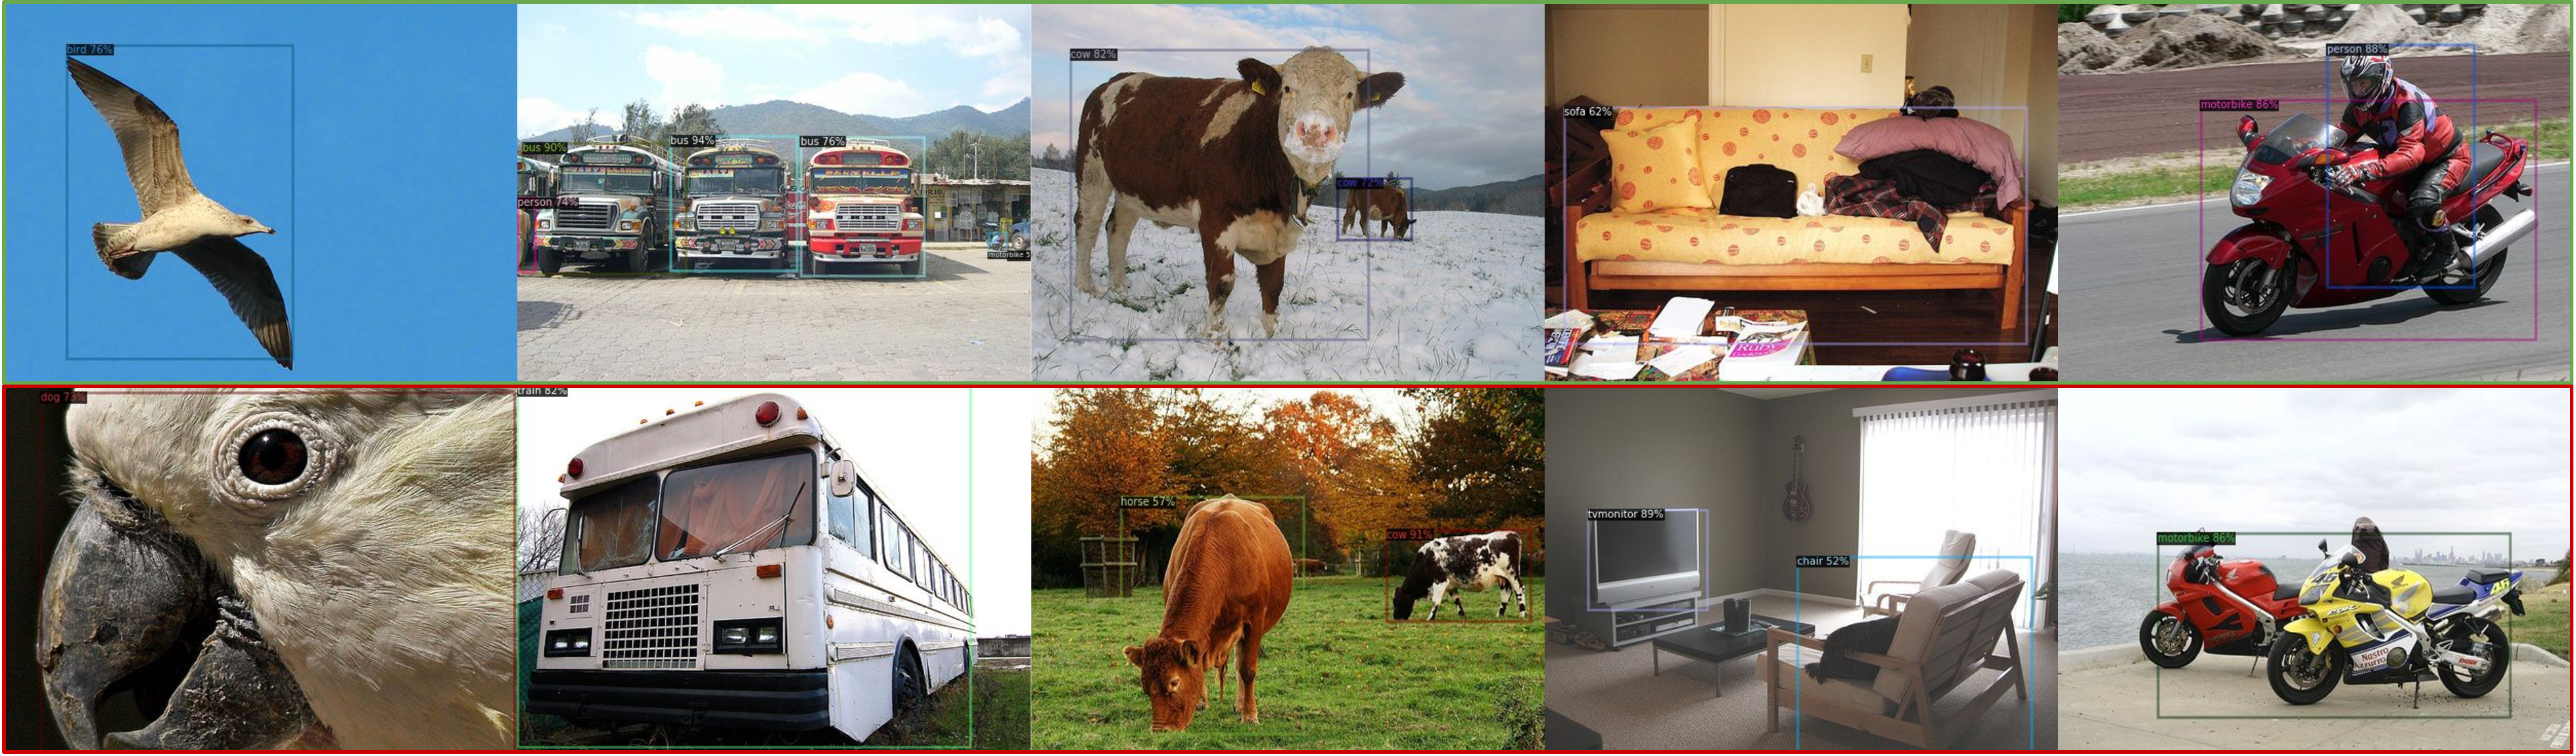
\includegraphics[width=.8\columnwidth*2]{figs/tfa_results.pdf}}
%     \caption{Detection results of our approach on novel classes (bird, bus, cow, sofa, and motorbike) from PASCAL VOC. We show success cases in the top row (green outline) and failure cases in the bottom row (red outline).}
%     \label{fig:det-vis}
%     \end{center}
%     \vspace{-8mm}
% \end{figure*}

\begin{figure*}[ht]
	\begin{center}
		\centerline{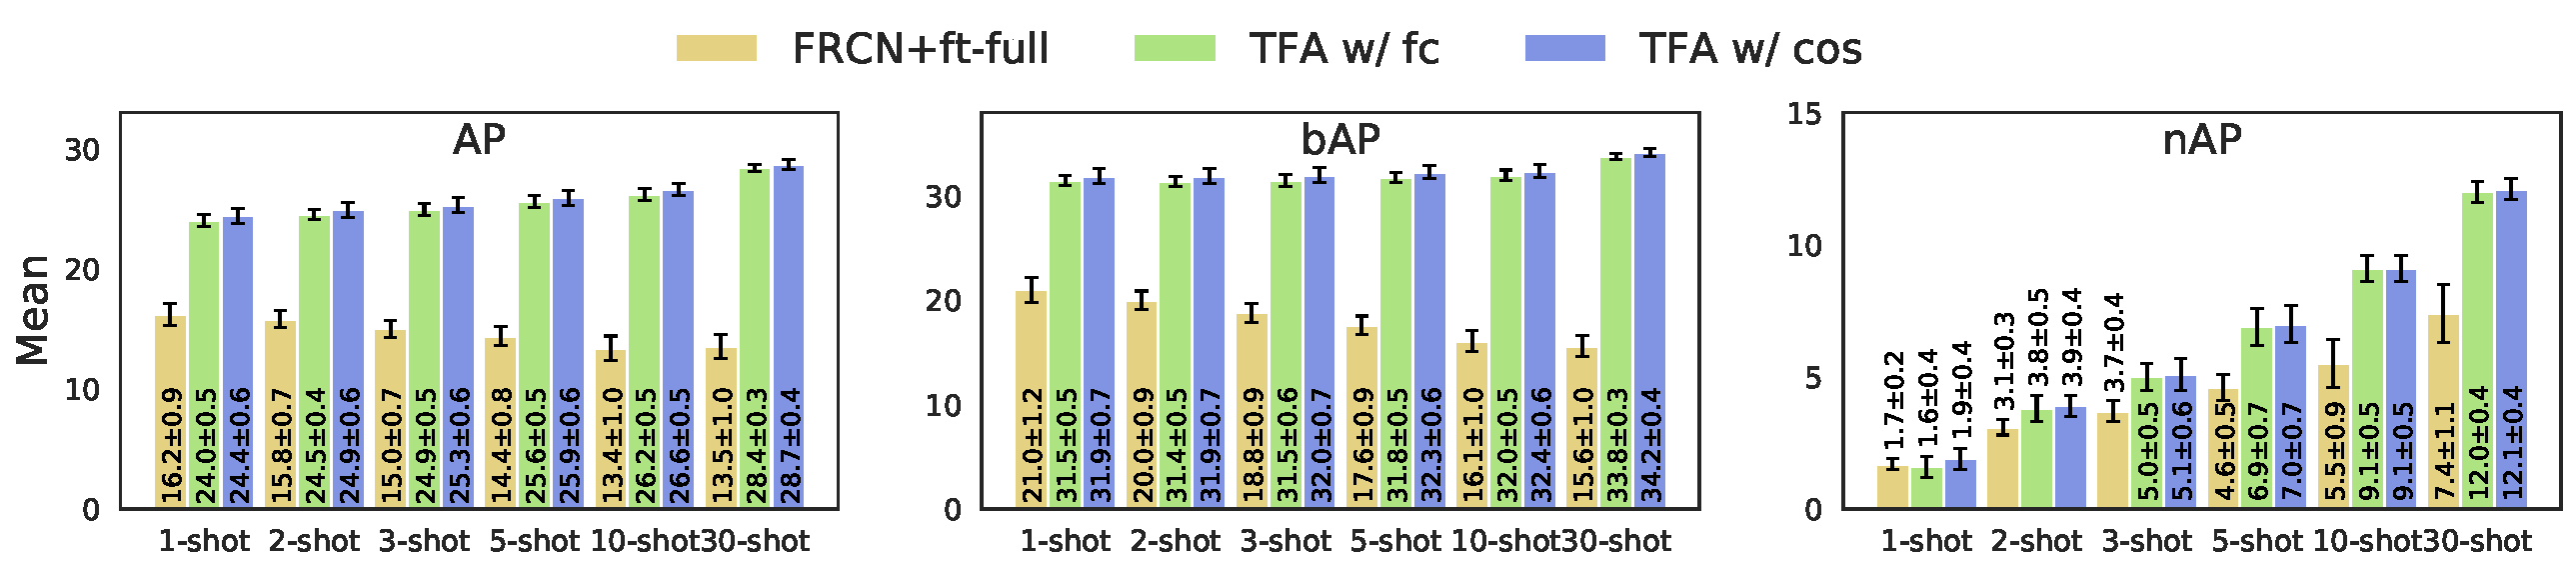
\includegraphics[width=.9\linewidth]{figs/coco_benchmark_full.pdf}}
		\vspace{-5mm}
		\caption{Generalized object detection benchmarks on COCO. For each metric, we report the average and 95\% confidence interval computed over 10 random samples.}
		\label{fig:coco_bench}
	\end{center}
\end{figure*}

{% \renewcommand{\arraystretch}{0}
\begin{figure*}[!ht]
	\centering
	\footnotesize
	\setlength{\tabcolsep}{0.1em}
	\adjustbox{width=.95\linewidth}{
		\begin{tabular}{ccccccc}
			\multirow{2}{*}{\rotatebox{90}{COCO}} &
			\rotatebox{90}{\hspace{4mm}Success} &
			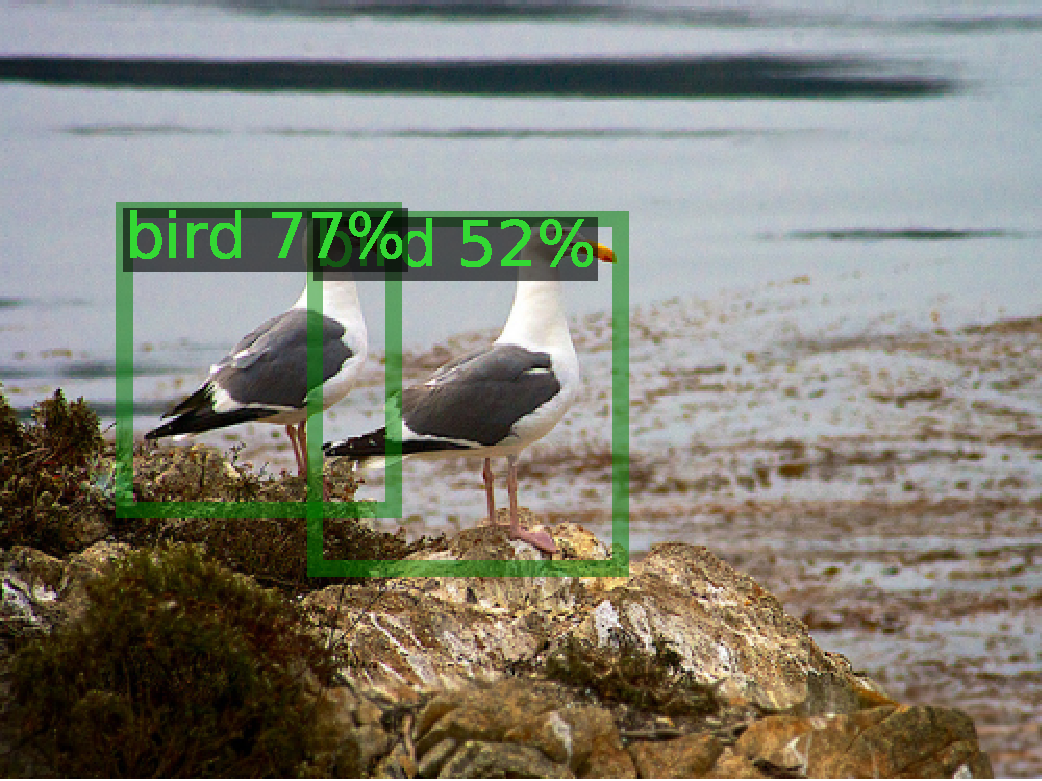
\includegraphics[width=1in]{figs/coco_bird_a.pdf} & 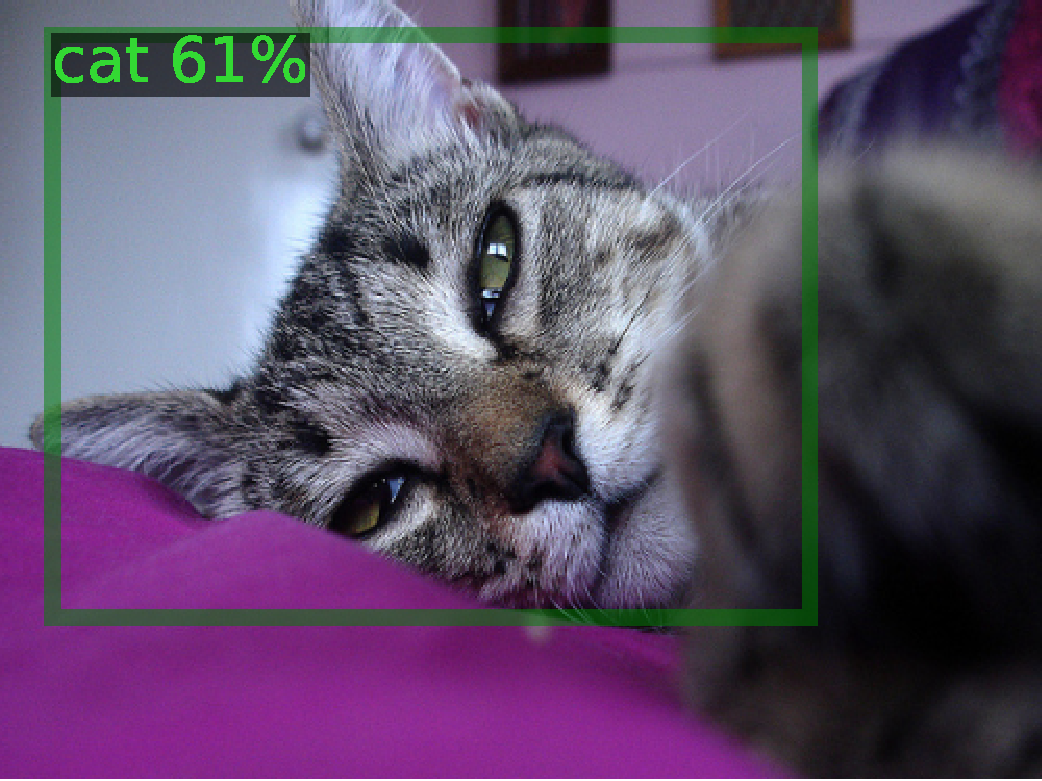
\includegraphics[width=1in]{figs/coco_cat_a.pdf} & 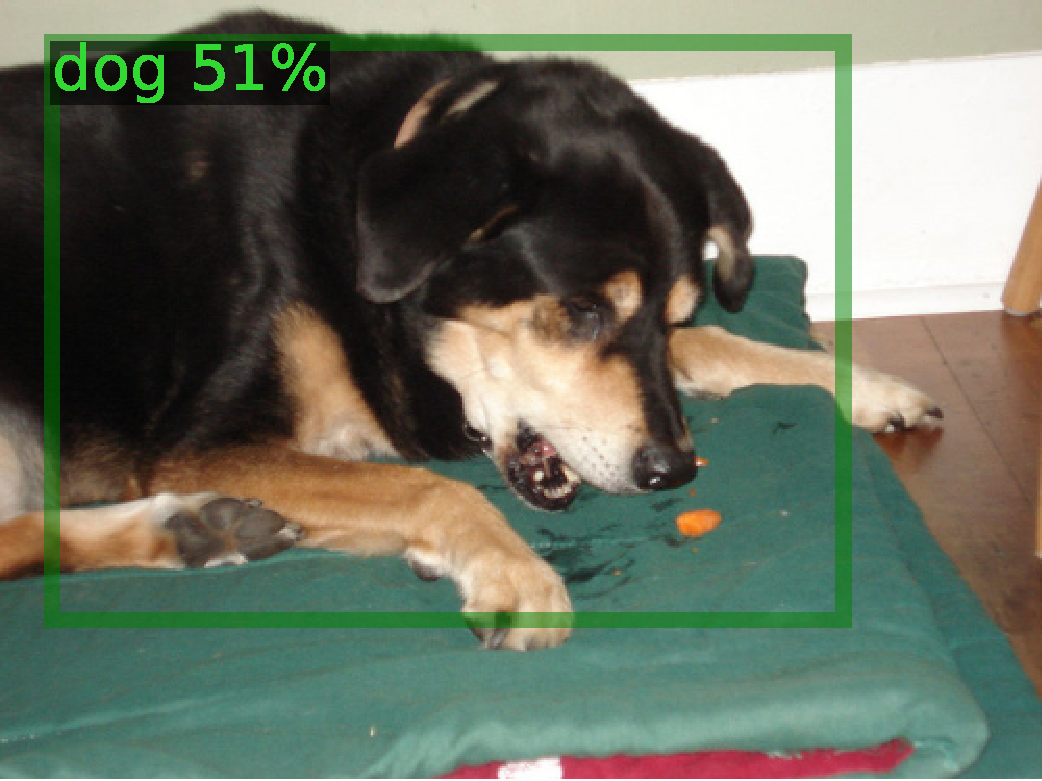
\includegraphics[width=1in]{figs/coco_dog_a.pdf} & 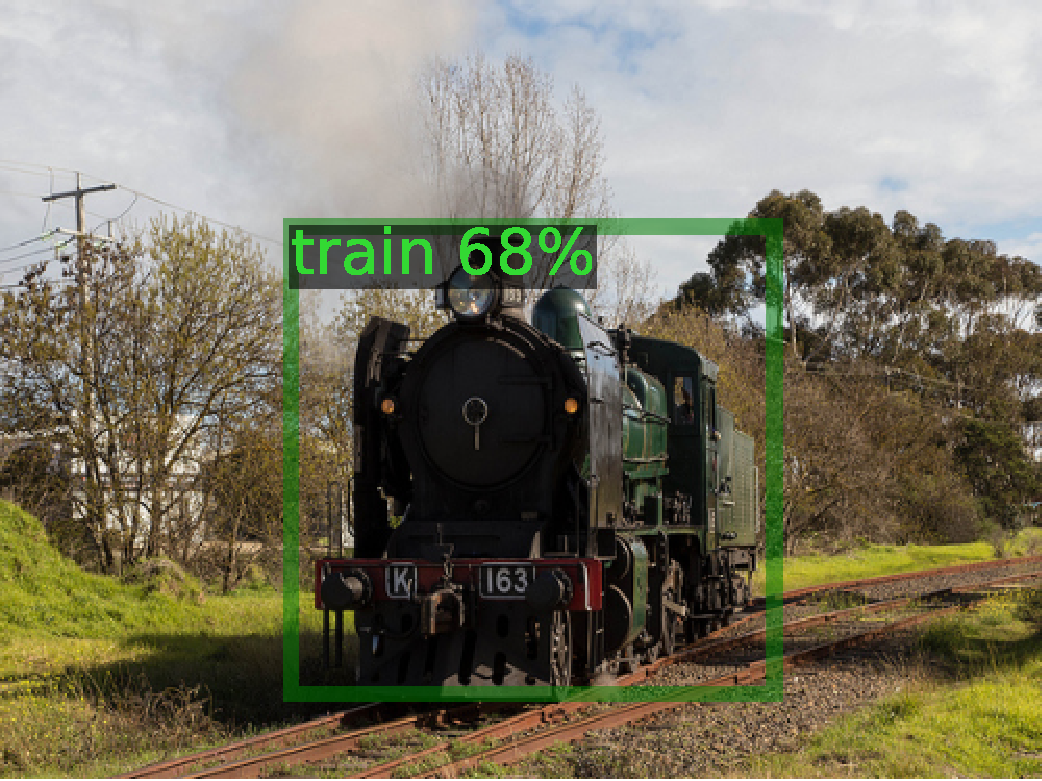
\includegraphics[width=1in]{figs/coco_train_a.pdf} & 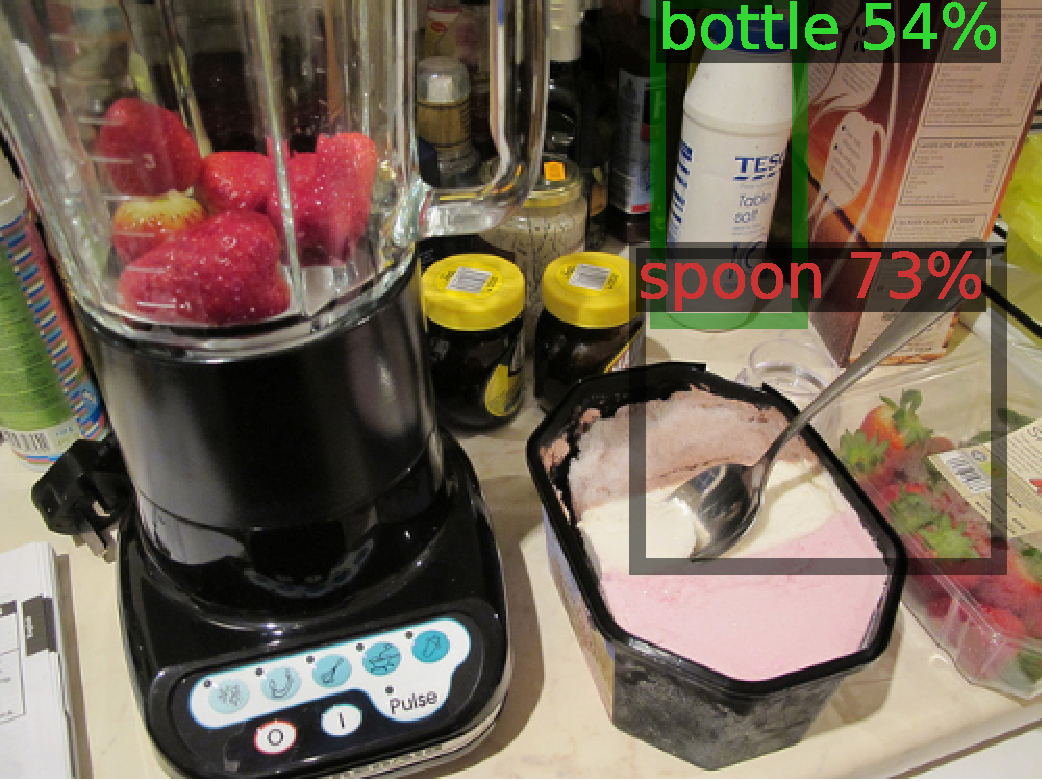
\includegraphics[width=1in]{figs/coco_bottle_a.pdf} \\
			& \rotatebox{90}{\hspace{4mm}Failure} &
			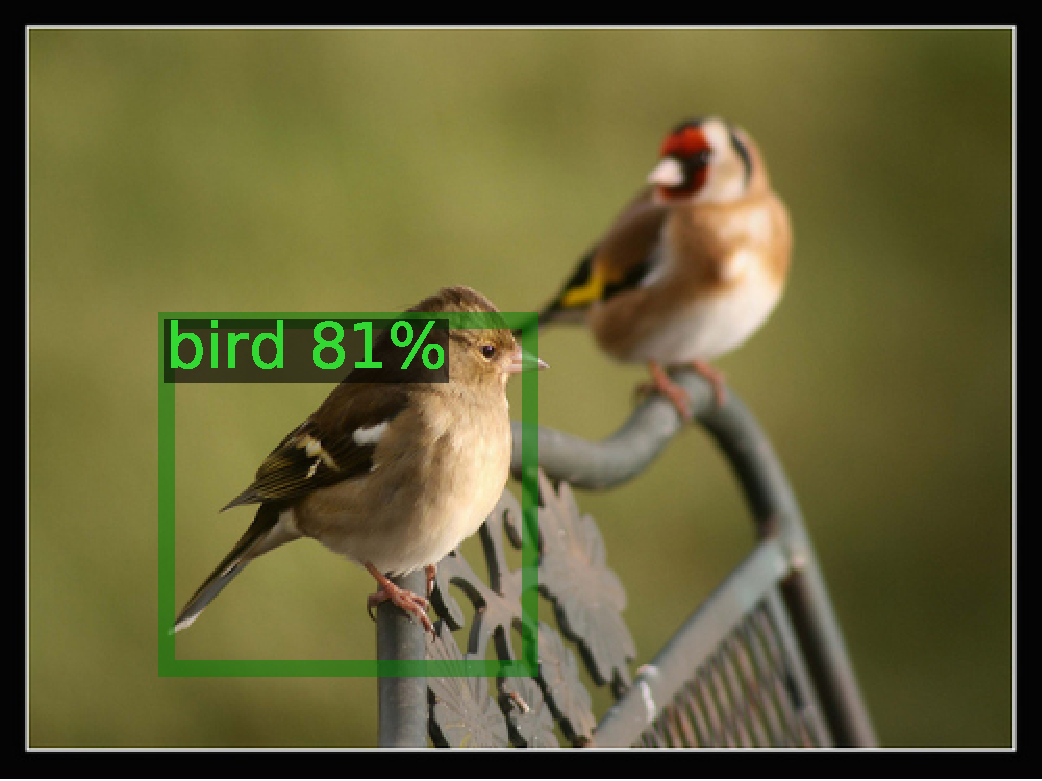
\includegraphics[width=1in]{figs/coco_bird_b.pdf} & 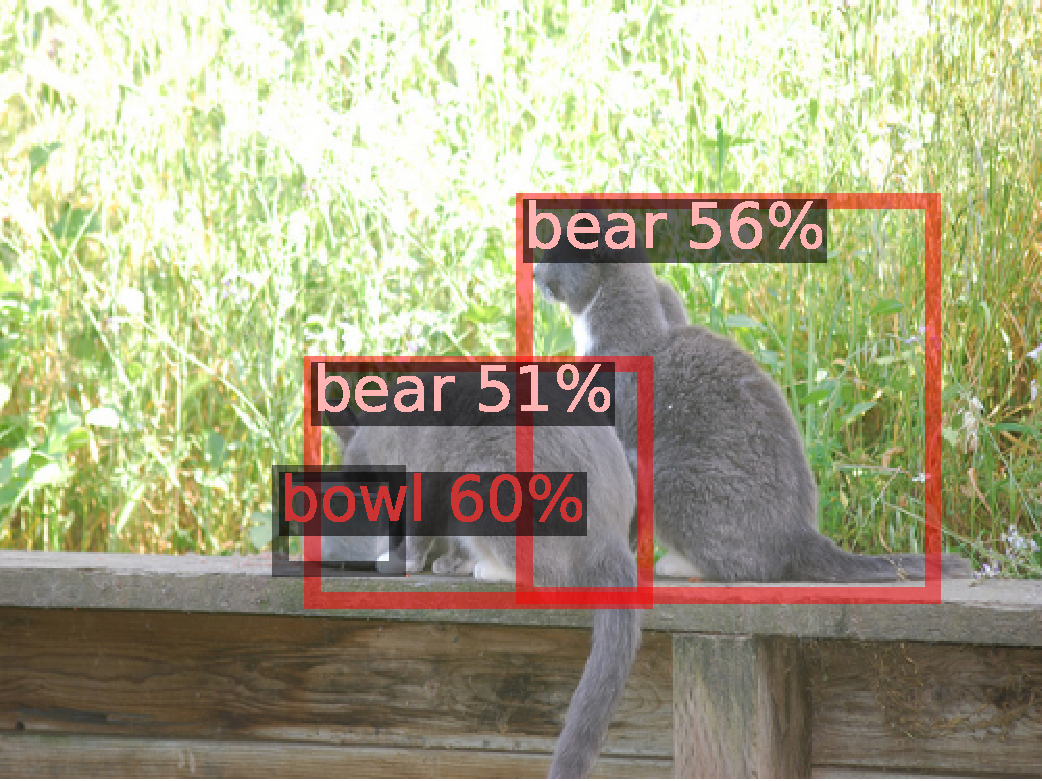
\includegraphics[width=1in]{figs/coco_cat_b.pdf} & 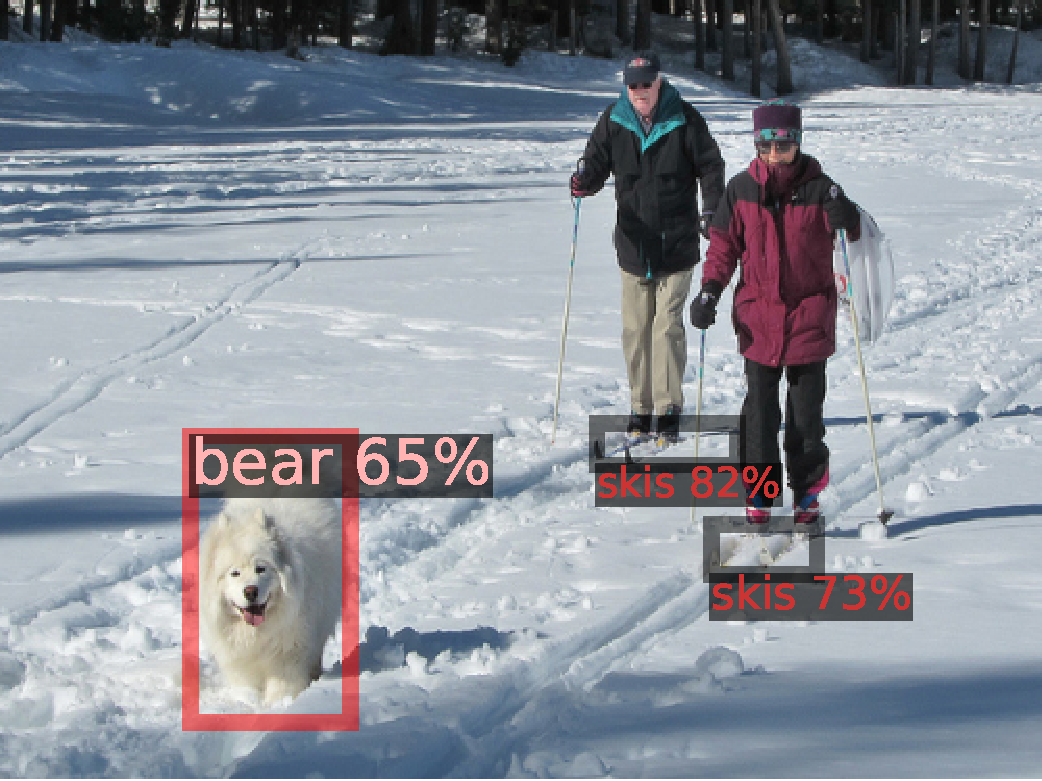
\includegraphics[width=1in]{figs/coco_dog_b.pdf} & 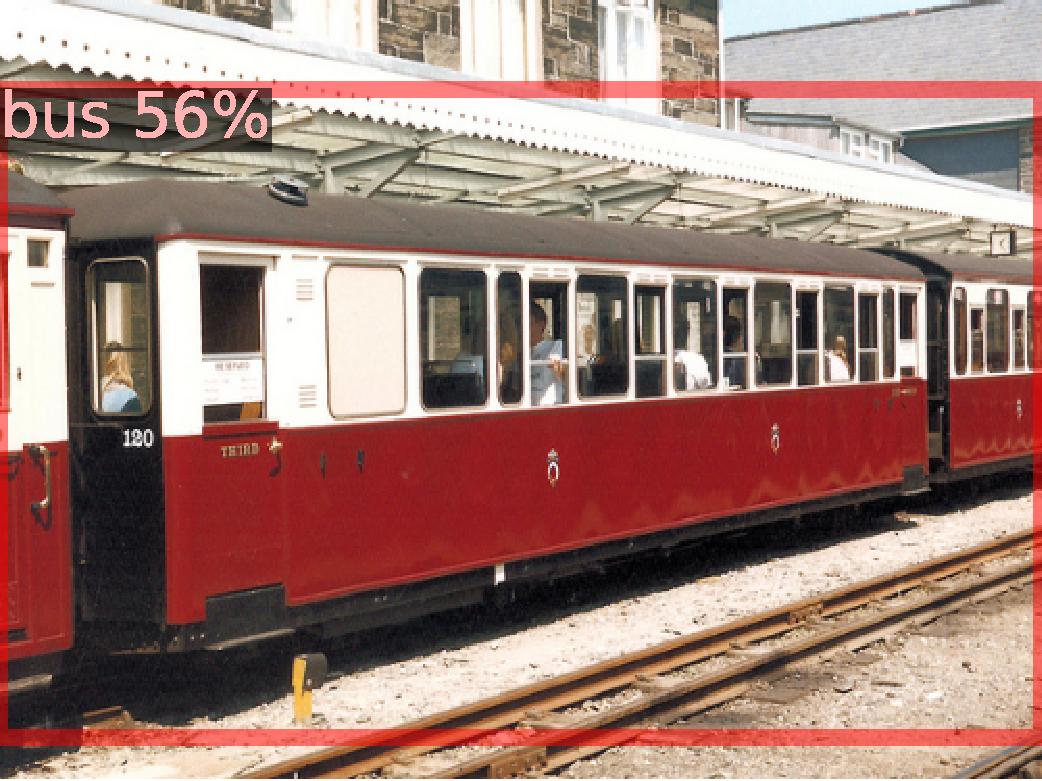
\includegraphics[width=1in]{figs/coco_train_b.pdf} & 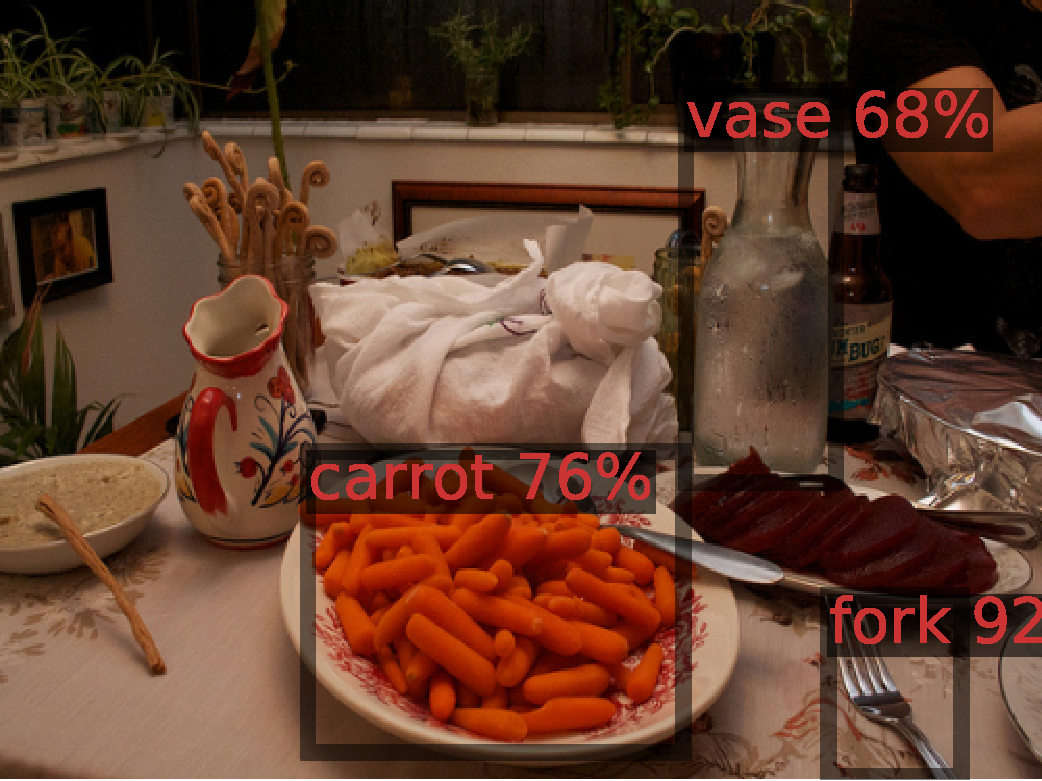
\includegraphics[width=1in]{figs/coco_bottle_b.pdf} \\
	\end{tabular}}
% 	\caption{Detection results of our approach on novel classes (bird, bus, cow, sofa, and motorbike) from PASCAL VOC. We show success cases (green boxes) in the top row and failure cases (red boxes) in the bottom row. \vspace{1mm}}
    \caption{Success (green boxes) and failure (red boxes) cases of our approach on novel classes from COCO (bird, cat, dog, train, and bottle). The black boxes are detected objects of irrelevant classes, which can be ignored. \vspace{1mm}}
    \label{fig:det-vis}
\end{figure*}}

% \minisection{More random samples.}
% On the current few-shot object detection benchmarks, performance numbers are reported and compared on a single random sample of training shots.
% However, since only a few examples are available, these numbers have high variance, and the differences in performance may vary greatly from sample to sample, thus making the comparisons unreliable.
% To address this issue, we train our models on multiple random samples of training shots to obtain means and confidence intervals, which are used for better comparisons.
% In Figure~\ref{fig:avg-ap}, we show the cumulative mean and 95\% confidence interval across 40 repeated runs on four different shots on the first split of PASCAL VOC.
% Although the performance is high on the first random sample, the average decreases significantly as more samples are used.
% Additionally, the confidence intervals across the first few runs are large, especially in the low-shot scenario.
% When we use more repeated runs, the averages stabilizes and the confidence intervals become small, which allows for better comparisons.
% On PASCAL VOC, we use 30 repeated runs. \xin{maybe combine with the comments above and shorten or split this paragraph. }

% \minisection{Inclusion of base categories.}
% We additionally evaluate our models on base categories and report AP measures on base categories as well as the mean across both novel and base categories.
% Data distributions in the real world are naturally long-tailed, and the goal of few-shot vision systems should be to achieve high accuracy on novel categories while maintaining performance on base categories.

\subsection{Ablation study and visualization}
\label{sec:vis}

\minisection{Weight initialization.}
We explore two different ways of initializing the weights of the novel classifier before few-shot fine-tuning: (1) random initialization and (2) fine-tuning a predictor on the novel set and using the classifier's weights as initialization. We compare both methods on $K=1,3,10$ on COCO and show the results in Table~\ref{tab:weight_init}. 
On COCO, using the novel weights can improve the performance over random initialization. This is probably due to the increased complexity and number of classes of COCO. We use novel initialization for all COCO and LVIS experiments.

\minisection{Scaling factor of cosine similarity.}
We explore the effect of different scaling factors for computing cosine similarity. We compare three different factors, $\alpha=10,20,50$. We use the same evaluation setting as the previous ablation study and report the results in Table~\ref{tab:cos_scale}. On COCO, $\alpha=20$ achieves better novel AP at the cost of worse base AP. Since it has the best performance on novel classes across both datasets, we use $\alpha=20$ in all of our experiments with cosine similarity.


\begin{table}[!h]
	\centering
	\footnotesize
	\setlength{\tabcolsep}{0.4em}
	%\caption{Ablation of weight initialization of the novel classifier before few-shot fine-tuning. We compare random initialization (Random) and initialization using fine-tuned novel weights (Novel). \vspace{1mm}}
	% We evaluate using base and novel AP on 1/3/10 shots on split 3 of PASCAL VOC and COCO.
	\caption{Ablation of weight initialization of the novel classifier. \vspace{2mm}}
	\adjustbox{width=.9\linewidth}{
		\begin{tabular}{ccccc|ccc}
% 			\toprule
			\multirow{2}{*}{Dataset}&\multirow{2}{*}{Init.}&\multicolumn{3}{c|}{Base AP} & \multicolumn{3}{c}{Novel AP}\\
			& & 1 & 3 & 10 & 1 & 3 & 10 \\ \midrule
			\multirow{2}{*}{COCO} & Random & 34.0 & \textbf{34.7} & \textbf{34.6} & 3.2 & 6.4 & 9.6 \\ 
			& Novel & \textbf{34.1} & \textbf{34.7} & \textbf{34.6} & \textbf{3.4} & \textbf{6.6} & \textbf{9.8} \\
			\bottomrule
	\end{tabular}}
	\label{tab:weight_init} 
\end{table}

\begin{table}[!h]
	\centering
	\footnotesize
	\setlength{\tabcolsep}{0.4em}
	\caption{Ablation of scaling factor of cosine similarity. \vspace{1mm}}
	\adjustbox{width=.9\linewidth}{
		\begin{tabular}{ccccc|ccc}
% 			\toprule
			&&\multicolumn{3}{c|}{Base AP} & \multicolumn{3}{c}{Novel AP}\\
			Dataset & Scale  & 1 & 3 & 10 & 1 & 3 & 10 \\ \midrule
			\multirow{3}{*}{COCO} & 10 & \textbf{34.3} & \textbf{34.9} & \textbf{35.0} & 2.8 & 3.4 & 4.7 \\ 
			& 20 & 34.1 & 34.7 & 33.9 & \textbf{3.4} & \textbf{6.6} & \textbf{10.0} \\
			& 50 & 30.1 & 30.7 & 34.3 & 2.4 & 5.4 & 9.0 \\
			\bottomrule
	\end{tabular}} 
	\label{tab:cos_scale}
\end{table}

\minisection{Detection results.}
We provide qualitative visualizations of the detected novel objects on COCO in Figure~\ref{fig:det-vis}.
We show both success (green boxes) and failure cases (red boxes) when detecting novel objects for COCO to help analyze the possible error types.
On COCO, we visualize the results of the 30-shot \texttt{\model w/cos} model.
The failure cases include misclassifying novel objects as similar base objects, \textit{e.g.}, row 2 columns 1, 2, 3, and 4, mislocalizing the objects, \textit{e.g.}, row 2 column 5, and missing detections, \textit{e.g.}, row 4 columns 1 and 5.
% We visualize the success and failure cases of our 10-shot \model w/ cos model on novel objects from the first split of PASCAL VOC in Figure~\ref{fig:det-vis}.
% Some failure cases include misclassifying novel objects as similar base objects, \textit{e.g.}, cow as horse, and identifying incorrect instance boundaries.

% In this section, we provide more qualitative visualization of the detected novel objects on Pascal VOC and COCO shown in Figure~\ref{fig:det-vis-sup}. We show both success (denoted by green boxes) and failure cases (denoted by red boxes) for each dataset to help analyze possible error types when detecting novel objects. The black boxes are detected objects of irrelevant classes, which can be ignored.  
% On PASCAL VOC, we visualize the results of the 10-shot \texttt{\model w/cos} model on novel objects from splits 2 and 3.
% On COCO, we visualize the results of the 30-shot \texttt{\model w/cos} model on novel objects.

% The failure cases shown in Figure~\ref{fig:det-vis-sup} could be misclassifying the object types(\textit{e.g.}, row 2 columns 1, 3, and 4), mislocalizing the objects (\textit{e.g.}, row 2 columns 2 and 5), and missing boxes (\textit{e.g.}, row 4 column 1 and row 6 columns 1 and 5).
